\documentclass[12pt,notitlepage,nofootinbib]{revtex4}
\usepackage{graphicx}
\usepackage{bm}
\usepackage{rotating}
\def\baselinestretch{1.2}
\usepackage{dcolumn}
\usepackage{times}
\usepackage{color}
\usepackage{amsmath} 
\usepackage{extarrows}
\usepackage{listings}
\usepackage{url}
\setlength{\mathindent}{0pt}

\begin{document}

\title{StochSS Hands-on Tutorial Series: 2 - Sensitivity Analysis with StochSS}

\author{StochSS Development Team}
\affiliation{Department of Computer Science - University of California, Santa Barbara}

\date{\today}

\maketitle

\section{\label{sec:pre}Prerequisites}
\begin{itemize}
\item StochSS 1.4 (or later) installed on your computer (please follow download and installation instructions at \url{www.stochss.org}). 
\item A basic understanding of well mixed discrete stochastic simulations and models based on ordinary differential equations \cite{dan,sundials}. 
\item  A basic knowledge of the functionalities in the StochSS GUI (please consult the \textit{Basic Introduction to StochSS} tutorial).
\item The following login screen appears on your browser: please log in.
\end{itemize}

\begin{figure}[!htb]
\centering
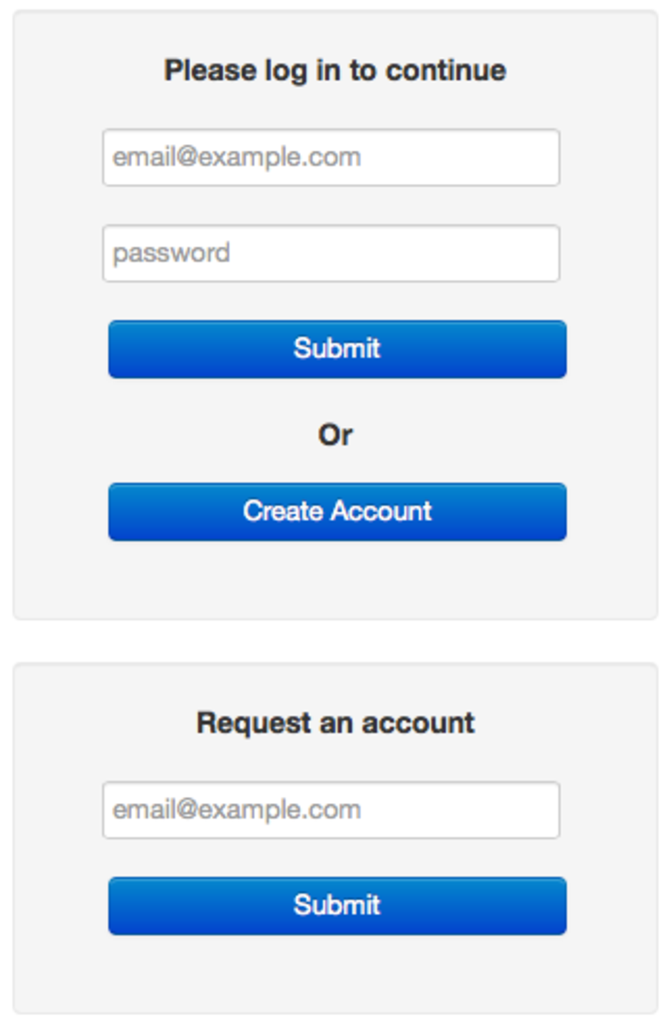
\includegraphics[scale=0.64]{user-login.pdf}
\end{figure}

\section{Forward Sensitivity Analysis}
StochSS implements forward sensitivity analysis for the deterministic (ODE-based) solver based on the SUNDIAL�s CVODES solver \cite{sundials}. The sensitivity analysis data generated by StochSS are unscaled (and so are the sensitivity analysis plots within the StochSS GUI).

\section{An Instructive Example}
We consider the Michaelis-Menten model that can be imported from the StochSS Public Library (see the \textit{Introduction to StochSS} tutorial for instructions on how to import models in StochSS). Details on the Michaelis-Menten model can be found at the following URL: \url{http://en.wikipedia.org/wiki/Michaelis-Menten_kinetics}

The snapshot below is from the StochSS simulation page. \textbf{\textit{mm}} is the unique name we assigned to the imported Michaelis-Menten model. We perform sensitivity analysis only on the relevant parameters of the model: \textit{mu, k3 Etot, Vmax} and \textit{Km}. On the \textcolor{blue}{Reactions} page of the  \textbf{\textit{mm}}  model it is easy to see that these are the only parameters that directly affect the values of the species \textit{S} and \textit{P}. Also, note on the same page that the parameter \textit{k3} directly affects only the dynamics of species \textit{P}.

\begin{figure}[!htb]
\centering
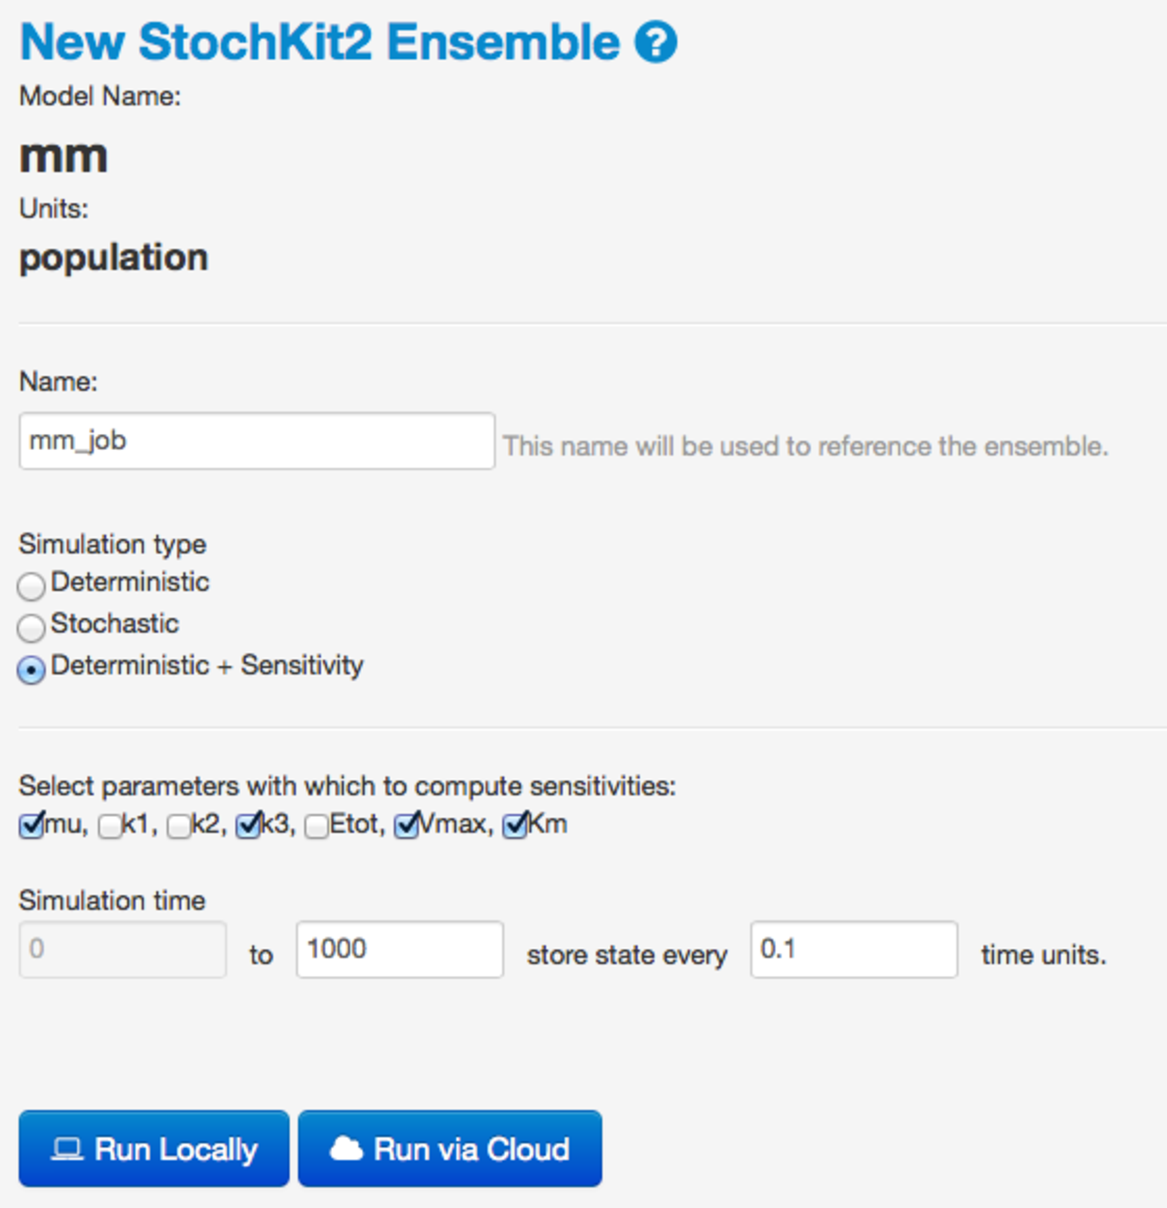
\includegraphics[scale=0.64]{sensi.pdf}
\end{figure}

\subsection{Scaling in sensitivity analysis}
Let�s consider the population of \textit{P} and the parameter \textit{Vmax} in our Michaelis-Menten model. The sensitivity of the rate of the increase in population \textit{P} to the parameter \textit{Vmax} is defined as the incremental rate of change in \textit{P} due to incremental changes in \textit{Vmax}:

\begin{equation}
\frac{\partial P(t)}{\partial V_{max}}.
\end{equation}

The analysis of the relative importance of various parameters in determining the dynamic behavior of a population can be negatively affected by the presence of different scales in the parameter set. Hence, for the purpose of comparison, it is preferable to consider scaled \textbf{sensitivities} (also called \textbf{elasticities}). The elasticity for species \textit{P} with respect to parameter \textit{Vmax} is defined as:

\begin{equation}
\frac{\partial P(t)}{\partial V_{max}} \cdot \frac{V_{max}}{P(t)} = \frac{\partial \log(P(t))}{\partial\log(V_{max})}.
\end{equation}

Using elasticities for parameter comparison is certainly an improvement with respect to the use of unscaled sensitivities. However, it is worth reminding that the use of elasticity may lead to artifacts \cite{scale}. After all, elasticity is just one possible transformation that can be applied to the sensitivities. An interesting discussion about sensitivity transformations in ecology is given in Ref.~\cite{scale}. \\
Among many possible transformation/scaling techniques, we would like to mention the \textbf{dimensionless scaled sensitivity} defined as \cite{calib}:

\begin{equation}
dss(t, V_{max}) = \frac{\partial P(t)}{\partial V_{max}} \cdot V_{max},
\end{equation}

and the \textbf{composite scaled sensitivity} defined as \cite{calib}:
\begin{equation}
css(t,V_{max}) = \sqrt \frac{\sum_{t=1}^N \left(dss(t,V_{max})\right)^2}{N},
\end{equation}
where $N$ is the number of observations.\\
Model simulation results will be more sensitive to parameters with larger \textit{elasticities}, \textit{css} and \textit{css} values.\\
The following simple \textit{octave/matlab} script uploads the data from a simulation run  \footnote{Please consult the \textit{Basic Introduction to StochSS} tutorial for instructions on how to download your simulation data.} (file \textit{output.txt}) of the Michaelis-Menten model, implements different scaling procedures and plots some of the results:

\newpage

\begin{verbatim}

x = dlmread('output.txt'); % loading the data file
t = x(5:size(x),1); % time array
N = size(t,1); % number of observations
St = x(5:size(x),2); % time series for S
Pt = x(5:size(x),3); % time series for P
% sensitivity analysis for S and P - Km, mu, Vmax, k3 
sensiS = x(5:size(x),[4,6,8,10]); 
sensiP = x(5:size(x),[5,7,9,11]);
% parameters - Km, mu, Vmax, k3
params = x(3,1:4); 
% scaling correction to avoid division by zero
deltaS = 0.0001 * (min(St(St(:, 1) > 0, 1))); 
deltaP = 0.0001 * min(Pt(Pt(:, 1) > 0, 1));
% dimensionless scaled sensitivity 
%(weight is 1 for all observations)
dssS = sensiS .* params; 
elasticityS = dssS ./ (St .+ deltaS); 
% composite scaled sensitivity
cssS = sqrt(sum(dssS .* dssS) ./ N); 
dssP = sensiP .* params;
elasticityP = dssP ./ (St .+ deltaP); 
cssP = sqrt(sum(dssP .* dssP) / N); 
figure(1)
plot(t,elasticityS)
title ('Elasticities for S');
xlabel('time');
legend('Km','mu','Vmax','k3','location','northwest');
figure(2)
plot(t,elasticityP)
title ('Elasticities for P');
xlabel('time');
legend('Km','mu','Vmax','k3','location','northeast');

\end{verbatim}

\newpage

\begin{thebibliography}{9}

\bibitem{dan}
  D.T. Gillespie.
  \textit{Exact stochastic simulation of coupled chemical reactions}.
  J. Phys. Chem., 81(25), 2340-2361 (1977)

\bibitem{sundials}
  A. C. Hindmarsh et al.,
  \textit{SUNDIALS: Suite of nonlinear and differential/algebraic equation solvers}.
  ACM Trans. Math. Softw., 31(3), 363-396 (2005)
  
  \bibitem{scale}
  W. A. Link and P. F. Doherty Jr.,
  \textit{Scaling in sensitivity analysis}.
  Ecology, 83(12), 3299-3305 (2002)
  
  \bibitem{calib}
  M. C. Hill,
  \textit{Methods and guidelines for effective model calibration}. 
  U.S. Geol. Surv. Water Resour. Invest. Rep. 98-4005 (1998)
  
\end{thebibliography}

\end{document}
